\section{Plant considered for system identification} \label{sec:plant_considered}
 
    % Gebruik dalk hierdie par erens??
    % \paragraph
    % As discussed in \ref{sec:linear_model}, the payload is attached near the CoM of the vehicle 
    % and has a minimal effect on the attitude dynamics.
    % The swing damping controllers are therefore applied in the translational velocity loop
    % and the original attitude controls are used for inner loop controllers.
    % Therefore the attitude state variables of the quadrtotor are excluded from the system identification model.

    % The model identified by DMDc or HAVOK will be used to design a longitudinal velocity controller.
    % As shown in \ref{fig:system_id_plant}, the plant considered for system identification includes the dynamics of the inner loop, attitude controllers.
    % The swing damping controllers which will utilise the identified model act only in the translational velocity loop.
    % Because of the large time-scale separation between the inner and outer loop controllers, 
    % the attitude states have a negilable effect on the plant dynamics seen by the velocity controller.
    % As discussed in Section~\ref{sec:linear_model}, the payload minimally effects the quadrotor attitude because it is attached near the CoM of the vehicle.
    % Therefore the attitude states are excluded from the system identification model.

    \paragraph
    Only the North velocity controller will be considered in this section. 
    Because of the symmetry of the quadrotor, this controller can then duplicated for East velocity control.
    The resulting input vector of the system identification plant is given by,
    \begin{equation}
        \bm{u} = \begin{bmatrix}
            A_{N,sp}
        \end{bmatrix} .
    \end{equation}
    For swing damping control, the controllers require state feedback from both the quadrotor and payload,
    hence the state vector of the considered plant is,
    \begin{equation}
        \bm{x} = \begin{bmatrix}
            V_N & \theta & \dot{\theta}
        \end{bmatrix}^T .
    \end{equation}
    % This is the state vector of the considered plant, 
    % but the controllers apply an augmented state vector that will be discussed in Chapter~\ref{chap:control_systems}.

    \paragraph
    Note that position is not included in the state vector because it does not affect the velocity controller.
    Also note that the inner loop controllers handle the attitude dynamics of the quadrotor.
    During pure longitudinal velocity setpoints the quadrotor experiences negligible altitude changes due the swinging payload.
    This is due to speed of the altitude controllers and the weak coupling between the payload angle and the altitude dynamics.
    The plant seen by the system identification process therefore mimics the common pendulum-on-a-cart model.
    A schematic of this 2D plant is shown in Figure \ref{fig:floating_pend}.
    In the following sections, simulations of the full quadrotor and payload system will be performed
    and different methods will be applied to identify different models of this plant.

    \begin{figure}[htb]
        \centering
        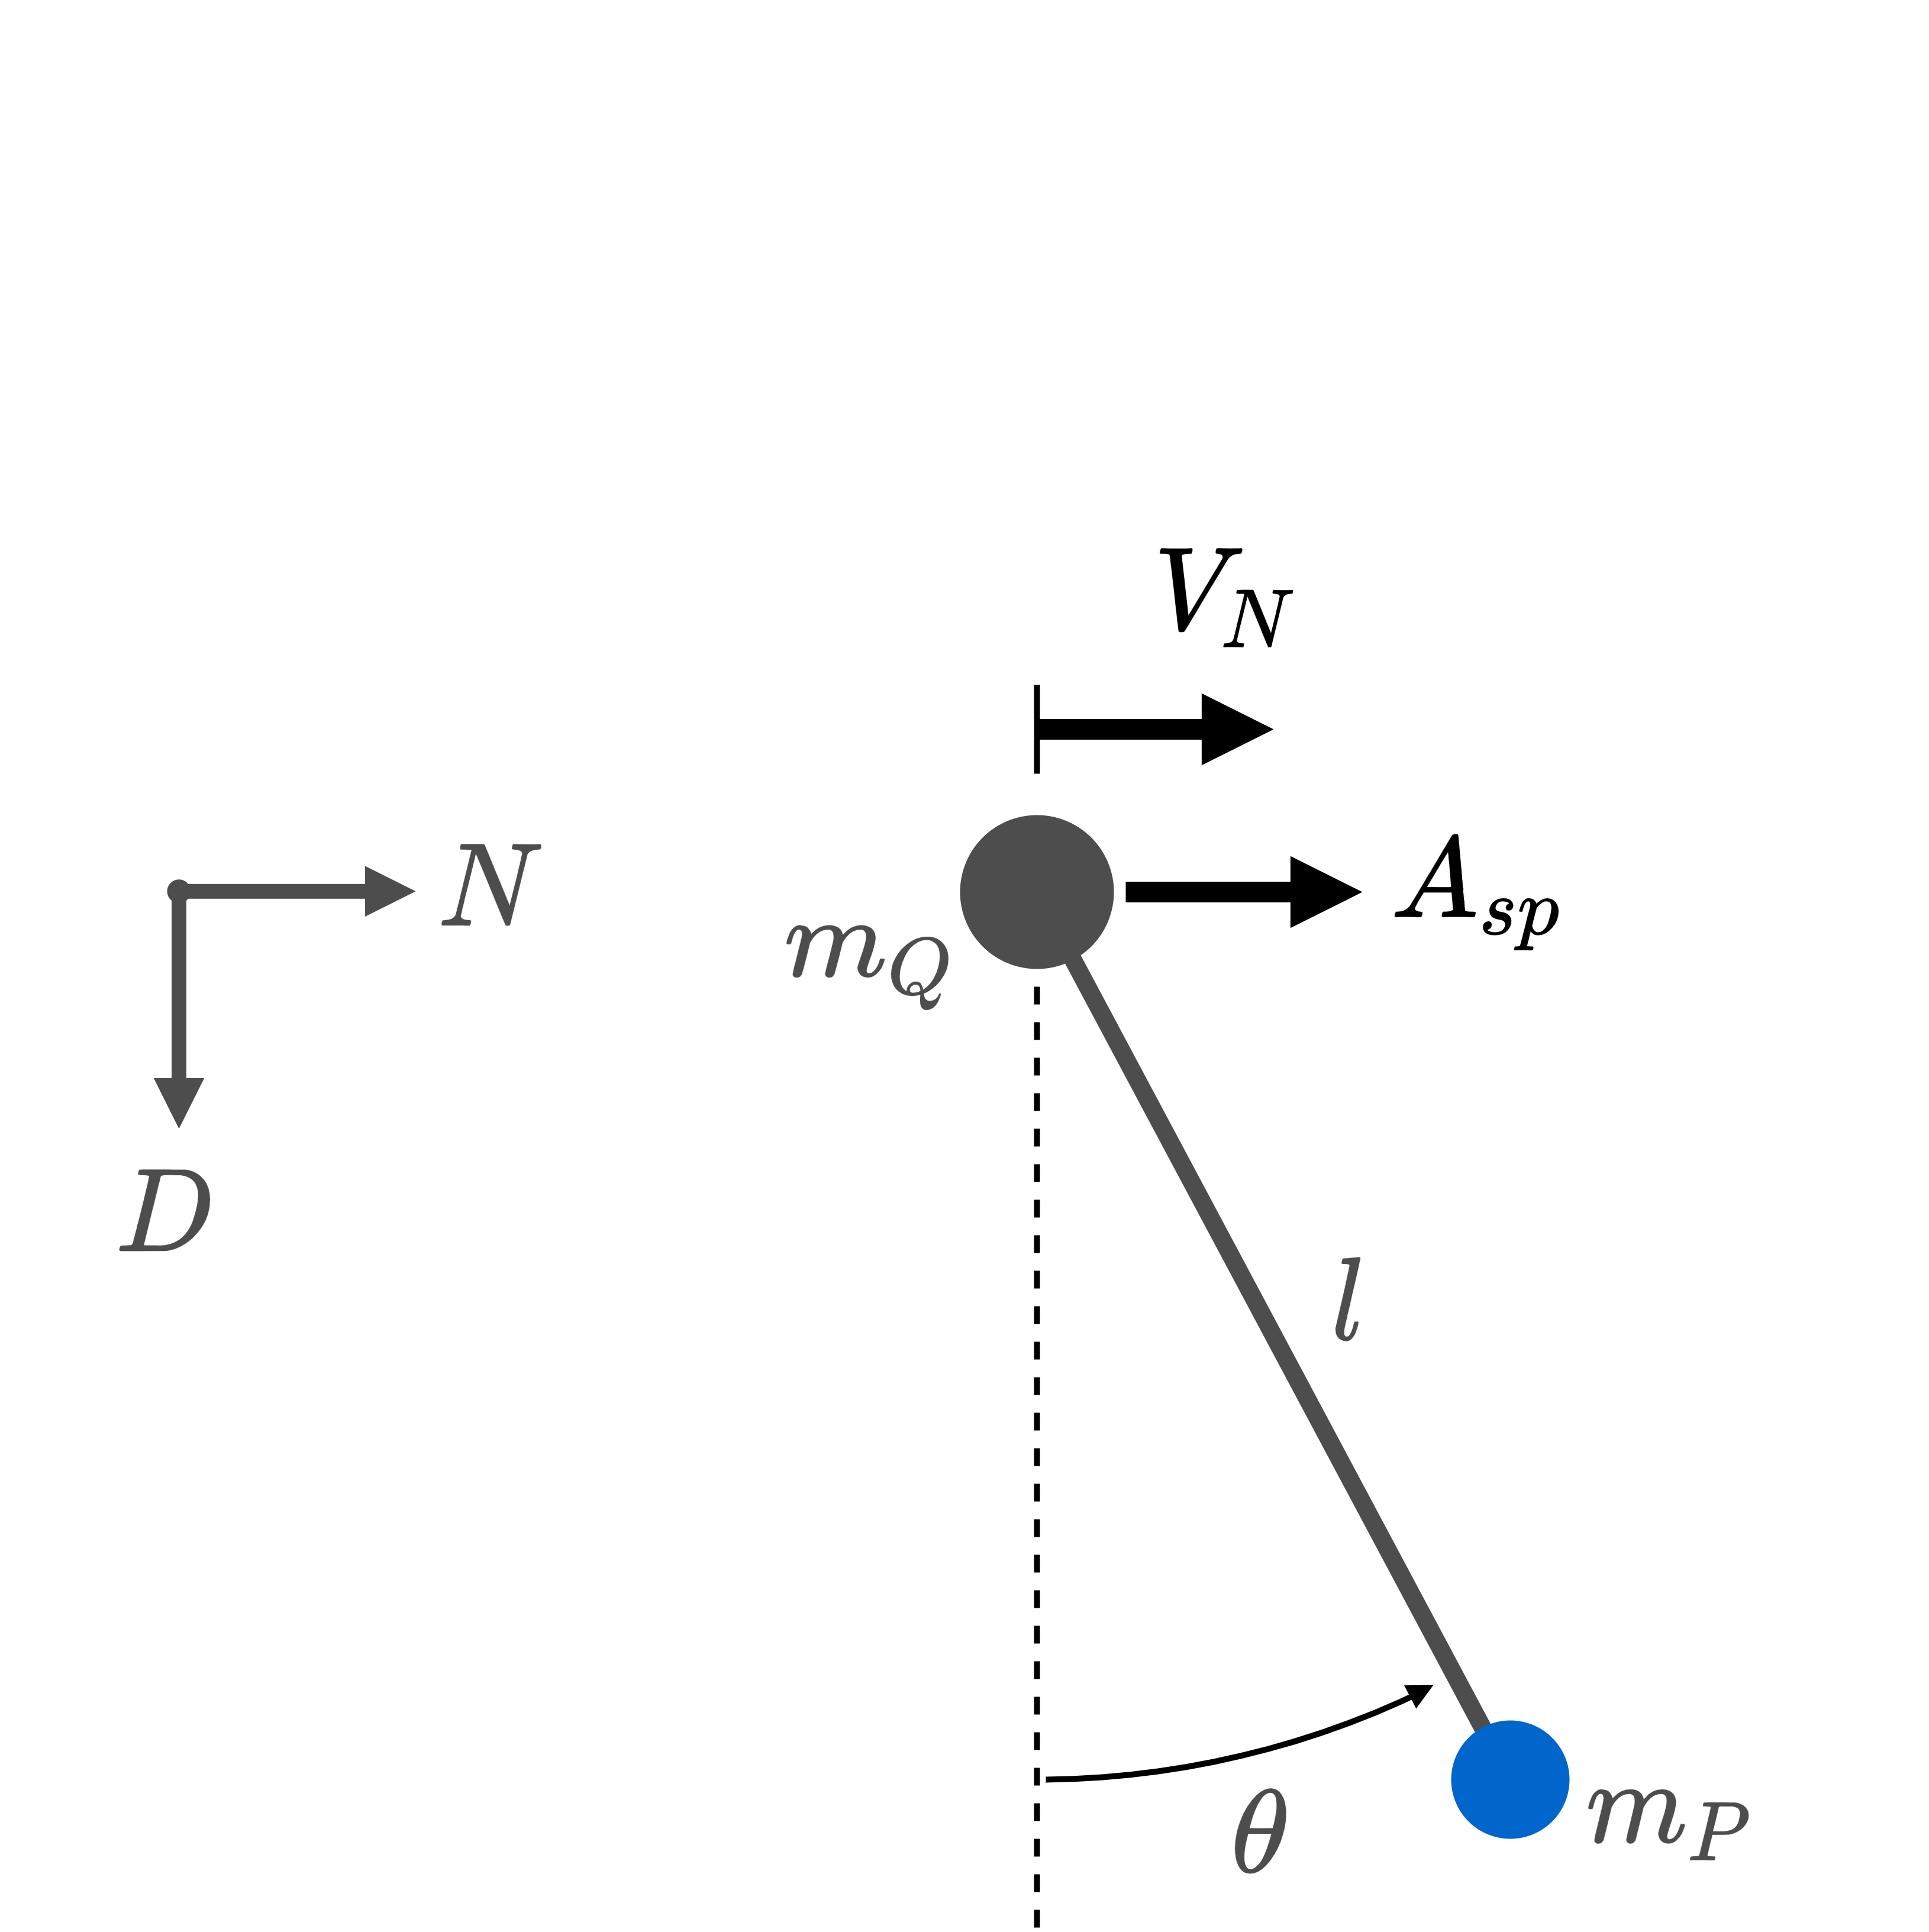
\includegraphics[width=0.45\linewidth]{floating_pend.png}            
        \caption{Schematic of a floating pendulum model considered for a North velocity controller}
        \label{fig:floating_pend}
    \end{figure}

    % The differential equations that describe the motion of this system 
    % were derived with Lagrangian mechanics in Chapter~\ref{chap:modelling}. 

    % From this derivation it is clear that the angular velocity of the payload, $\dot{\theta}$, is required to described the system dynamics.
    % However, $\dot{\theta}$ is not measured directly on the considered practical quadrotor setup.
    % Instead, the payload angle, $\theta$, is measured by a potentiometer attached to a ADC on Honeybee as described in Chapter \ref{chap:system_overview}.
    % As expected, this measurement is extremely noisy.
    % \murray{Maybe insert figure to show noise}
    % % Figure \ref{} shows the angle measurement during a practical experiment of the payload while Honeybee is held stationary
    % Numerical differentiation is applied to the noisy $\theta$ signal which results in a very inaccurate estimation of $\dot{\theta}$.
    % Therefore it is desirable to rather use $\theta$ in the system identification process. 

